\chapter{Methods} \label{chapMethod}
\section{Datasets}
There is a severe lack of forestry datasets which are publically available and were suitible for testing our approach. Therefore, a large portion of this work involved collecting our own data, or finding data from related fields to adapt to our domain.
\subsection{ Multi-Sensors Drone Data}
Many modern approaches to simultanous localization (SLAM) and semantic mapping require as input multiple sensing modalities, such as cameras, LiDAR, IMU, and GPS. Therefore, other members of our team build a modular, multi-sensor payload that could be mounted on a drone. A view of the payload can be seen in Figure \ref{fig:methods:payload}. 

\begin{figure}
    \centering
    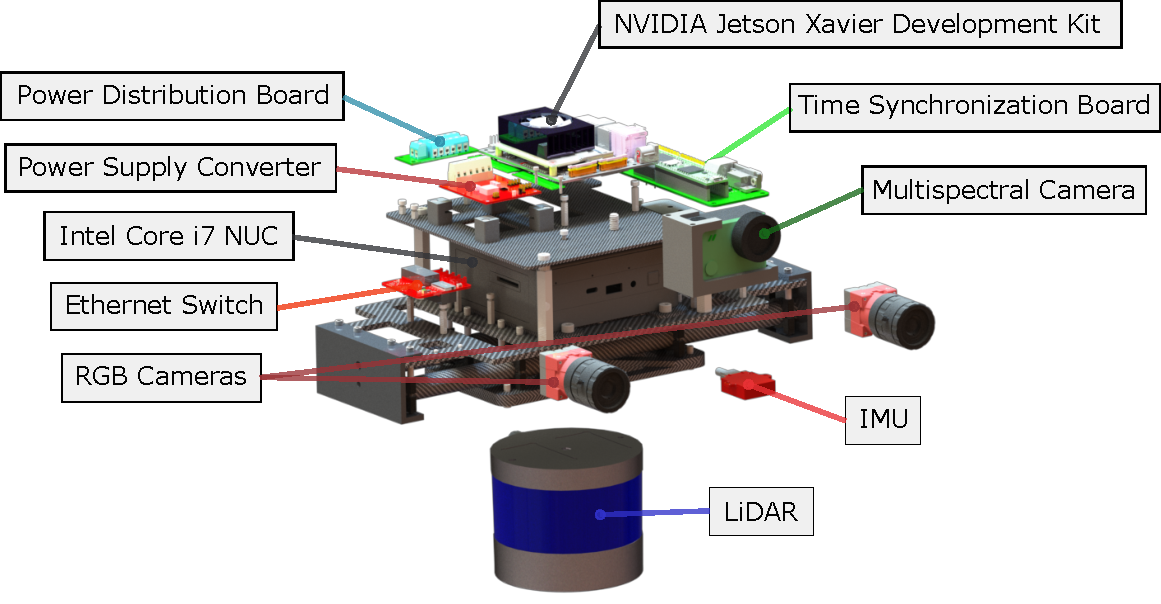
\includegraphics[width=\textwidth]{figs/methods/datasets/payload_annotated.pdf}
    \caption{The multi-sensor payload designed by our collaborators. This was used for collecting rich forestry drone data. Photo credit to Winnie Kuang.}
    \label{fig:methods:payload}
\end{figure}


\begin{figure}
    \centering
    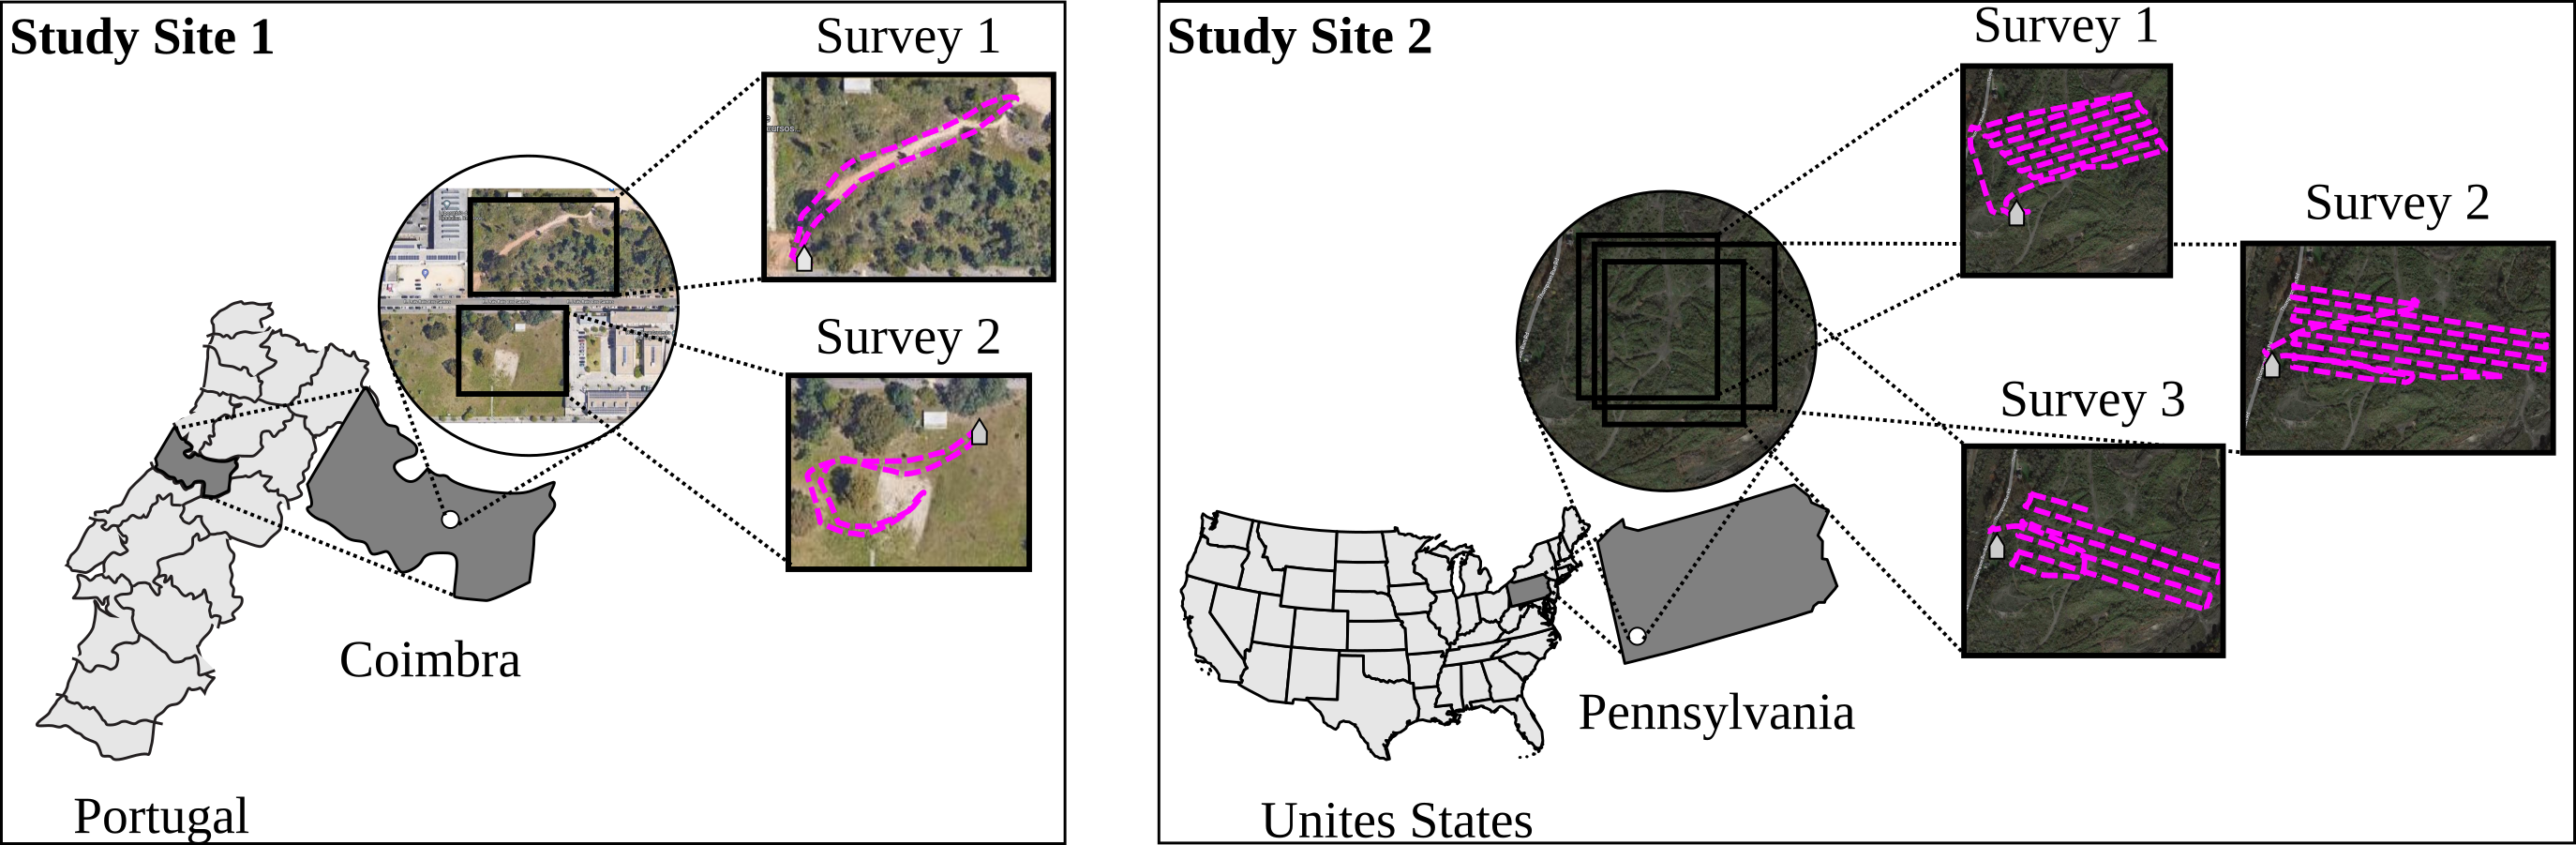
\includegraphics[width=\textwidth]{figs/methods/datasets/studySites1.png}
    \caption{Locations where we collected drone data. Photo credit to Francisco Yandun. TODO, consider updating to Oporto image if that's what the results are from.}
    \label{fig:methods:data_site}
\end{figure}

This payload is modular and could be mounted to different drones with different inclination angles. In these experiments, we used a DJI Matrice 600 and an AltaX Freefly, both large commercially-oriented drones with a high payload capacity. We flew a variety of different experiments, both under the canopy and over the canopy. In the under-canopy settings, we flew in small clearings between trees under manual control. Babak B. Chehreh from the University of Coimbra served as our pilot. In these experiments, we tried to survey the boundary of the clearing exaustively by using an oblique payload orientation of 30 degrees from horizontal.
\subsection{Commodity drone data}
Commodity drone data refers to data which can be acquired with only commercially-available tools and no specialized domain knowledge. In practice, a valuable and easy-to-collect source of data is GPS-tagged images collected in a pre-defined exhaustive survey. This can be obtained by even some of the smallest drones, such as DJI Mavic, which costs approximately \$1,600\footnote{\href{https://store.dji.com/product/dji-mavic-3-classic}{DJI Mavic}}. Commercial flight planners are a tool that allows a user to quickly define a survey region and fly over it in a geometric pattern. A common option is "lawnmower coverage" where a drone flies in a straight line, shifts over, and flies back the opposite direction. Another option is "grid coverage" where a lawnmower pattern is executed twice, in perpendicular directions. An important consideration when executing these surveys is the drone altitude, which represents a trade-off between coverage ability and spatial resolution. While drones can in theory fly to a substantial altitude, they are restricted in the US to 400ft and below due to concerns about interfering with crewed aircraft. The final consideration is front- and side-overlap. Front overlap refers to the fraction of the image which is observed in two consecutive frames captured as the drone is flying forward. The side overlap refers to how much overlap there is between neighboring flight lines.

In this work, we use several sources of commodity-level drone data. The first is actually collected with our more sophisticated drone. In these experiments, we only use the images from one camera and geotag them with our payload GPS. This is a reasonable analog for commodity drone data, since our camera and GPS are comprable to what would be found on a small commodity platform. 

The second source of data is taken from a study of structurally-complex western conifer forests \cite{Young2022OptimizingForests}. This data was collected with a DJI Mavic at an altitude

\subsection{Optical remote sensing data}
Optical remote sensing data is captured by cameras onboard satellites or airplanes. This class of data is extremely powerful because it enables understanding at planetary scales, often with no or low cost to the data consumer. Remote sensing data can take many forms such as LiDAR, synthetic aprature radar (SAR), and optical. In this work, we focus on optical data, since it is conceptually most similar to what we capture from drones. This data is collected by an electro-optical sensor which takes images of the earth. Then, the images are registered together and referenced into absolute geospatial coordinates. This process relies on the estimated pose of the platform when the image was taken, the height of the ground, and manual corrections. From there, an orthographic render is generated. This is a projection of the data into a top-down view, which is commonly aligned with the cardinal axes of the earth. Many satellite data sources capture bands outside of the visible wavelength. Sensors which capture a x to y number of bands are termed multispectral and sensors which capturer y to z bands are termed hyperspectral. In this work, we focus primarily on data collected by the National Aerial Imagery Program (NAIP) multispectral data source which contains red, blue, green and near-infrared bands.

\section{Geometric understanding of forests using drone data}
\subsection{SLAM}
TODO talk about the work that others did

\subsection{Photogrametry}
\begin{itemize}
    \item We use commercial solvers such as Metashape
    \item The images are initialized with the GPS coordinates
In general, commodity drones produce only monocular images with potentially a low-accuracy GPS and orientation estimate. A common approach for estimating geometric from this type of data is photogrametry, also known as structure from motion or 3D reconstruction. The origins of photogrametry date back to WWII where it was a manual processed to estimate the geometry of structures from aerial images. Modern automated approaches began todo. Preliminary reconstructions of realistic large-scale scenes began with academic work such as \cite{Agarwal2009}. Over the last decade, numerous commercial and open-source software have been developed to accomplish the task. Some examples include
\begin{itemize}
    \item \textbf{Agisoft Metashape}:
    \item \textbf{COLMAP}:
    \item \textbf{OpenMVG}:
    \item \textbf{OpenDroneMap}:
\end{itemize}

The details vary by application and assumption, but a common pipline is the following. First, distinctive features are detected in each image. These represent small patches of pixels which are likely to be distinctive, such as corners and edges. Then, features are matched between images, based on the local appearance. 
Given these correspondences, multiple things can be estiated. The first is the location of these matched points in the 3D space, using triangulation between the cameras. The second is the location of the cameras. Finally, if the camera isn't accurately calibrated, it's common to estimate the parameters which describe how points in the world appear on the image. Given the interplay between all of these elements, it's critical to estimated them together in a global joint optimization. The class of techniques for solving this problem are termed bundle adjustment and are often build on iterative nonlinear least squeres. 

After these quantities are estimated, it's common to re-estimate the correspondences between images using the existing solution as a way to filter incorrect correspondes which are not consisent with the majority of other matches. These steps are often the focus of extensive engineering effort to improve the final performance. 

After this iterative process converges, the result is a sparse output consisting of the camera locations and calibration parameters as well as a sparse set of 3D locations. This sparse representation doesn't capture the full geometry of the scene, since only the most distinctive points are represented. Moreover, because it is a pointcloud, we cannot reason about which parts of the scene would obstuct or "occlude" the view of another one. To accomplish these tasks, we leverage the fact that many solvers can produce a mesh representation of the surface of the scene. A mesh is a common representation in computer vision and graphics, which consists of a set of 3D points connected by triangular faces. 

The process of mesh computation varies by solver. A common first step is to estimate the likely depth to the surface from each camera using color constancy. This means that for a set of posible distances, the observed color from that camera is checked against the color which would be observed by the other camera, if that were the true location of the surface. From this information, a predicted most likely depth surface is predicted for each pixel. Then, the predicted depth is combined across all cameras to produce a consistent 3D geometry. This is often done using a truncated signed distance function representation \cite{} 

\begin{figure}
    \centering
    \includegraphics{example-image-a }
    \caption{Camera estimation}
    \label{fig:sparse-reconstruction}
\end{figure}

These solvers are becoming increasingly robust, and are well-suited to reconstructing scenes captured by drone surveys because the same location is often seen across many images.

\section{Semantic mapping for forests}
\end{itemize}
\subsection{Semantic segmentation}
In the image domain, we use a segmentation network based on a transformer architecture called SegFormer \cite{segformer21}. Given the relatively low amount of real-world images in our training dataset, this network was especially suitable since it showed strong performance on benchmark datasets and good generalization capabilities. We trained this model using the default parameters used in the MMSegmentation \cite{MMSegmentation} implementation. 
\begin{itemize}
    \item We annotated images coarsely using VIAME
    \item We train segformer with the MMSegmentation framework
\end{itemize}
    
\begin{figure}
    \centering
    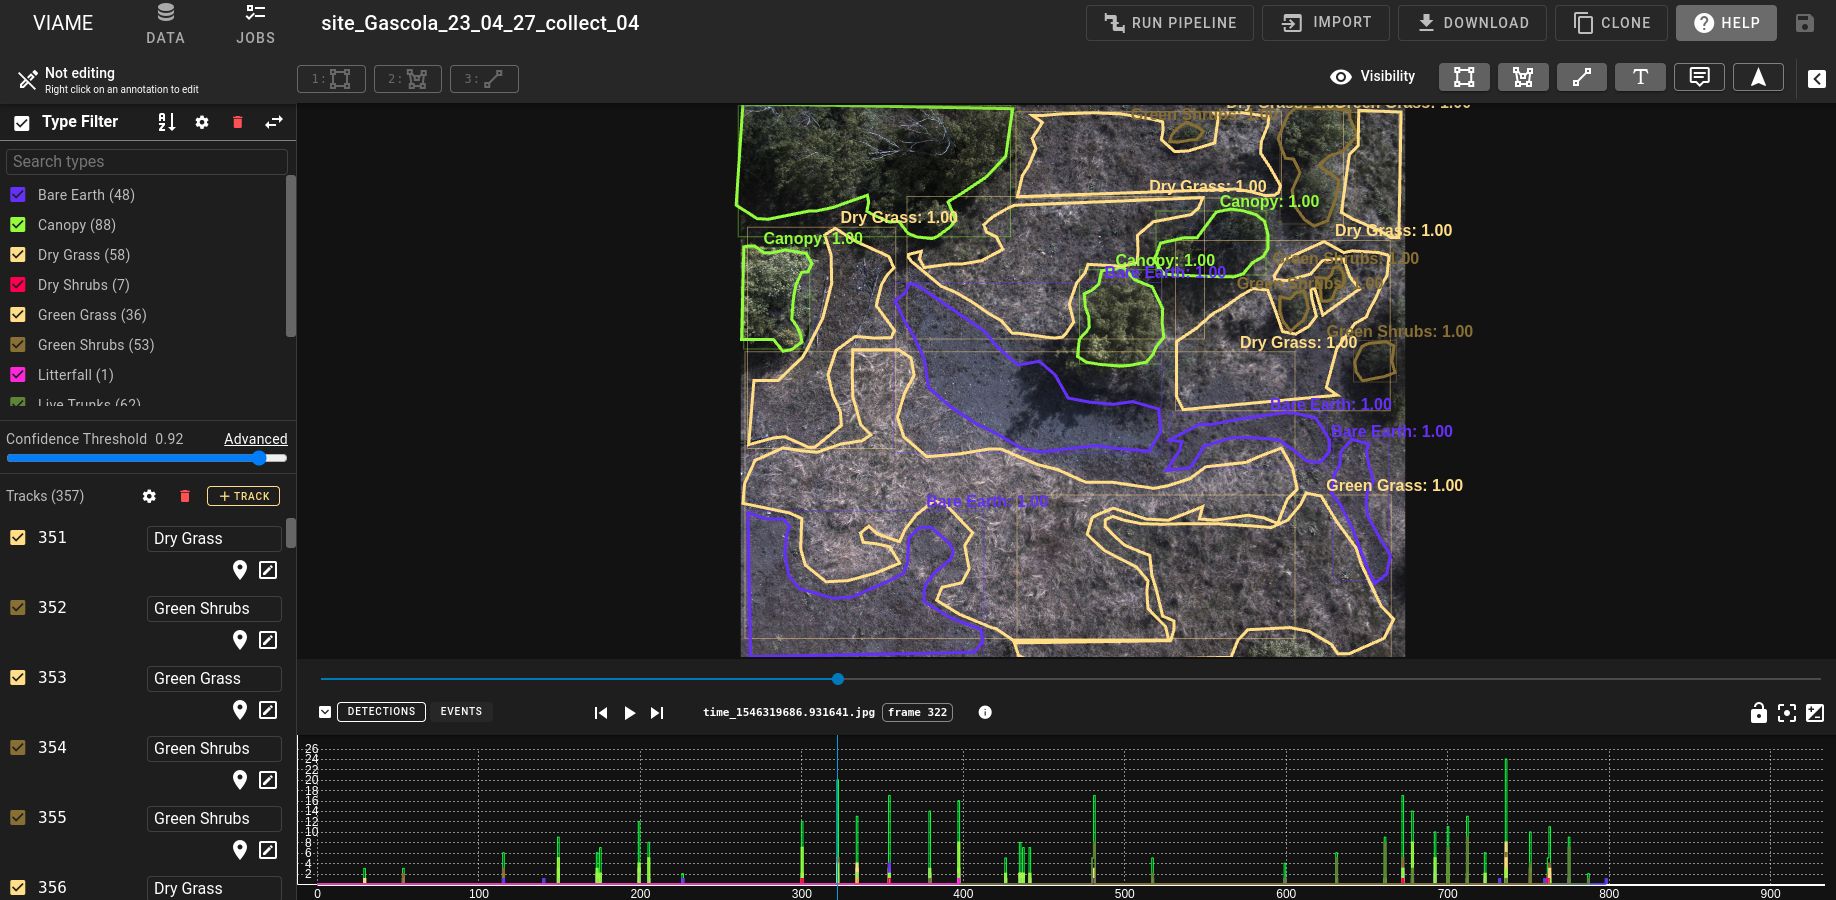
\includegraphics[width=\textwidth]{figs/methods/semantic_mapping/viame_example.png}
    \caption{Example manual annotations using the VIAME toolkit, a free and open source web annotator with potential support for integrated model training.}
    \label{fig:methods:manual-annotations}
\end{figure}

\subsection{LiDAR camera work}
\begin{itemize}
    \item Talk about the payload
    \item Talk about calibrating all the sensors
    \item Talk about the method
\end{itemize}

\begin{figure}
    \centering
    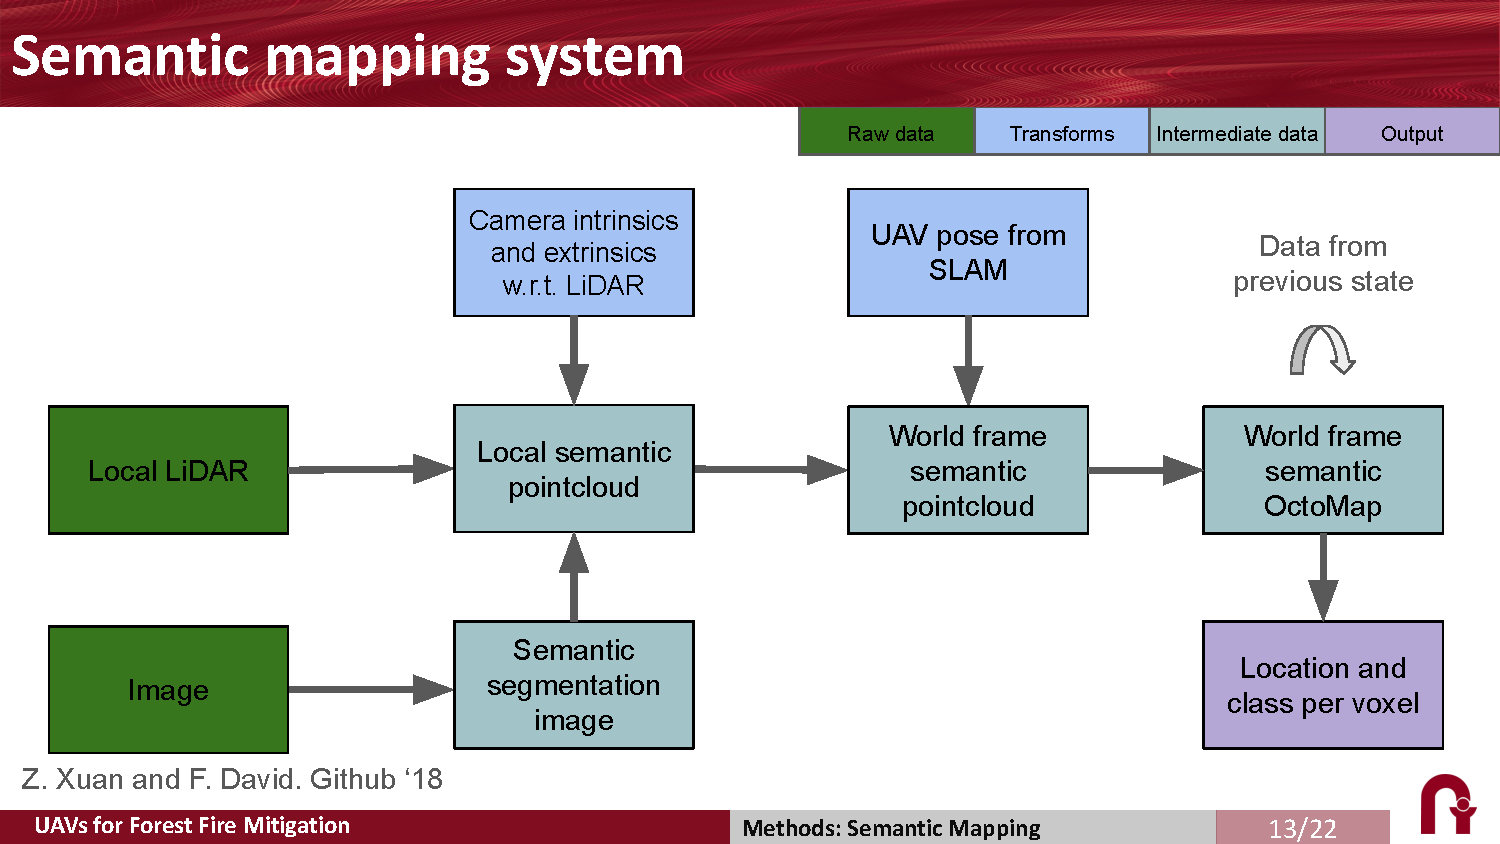
\includegraphics[width=\textwidth]{figs/methods/semantic_mapping/semantic_mapping_overview.pdf}
    \caption{An overview of the LiDAR-camera semantic mapping system}
    \label{fig:lidar-camera-semantic-mapping}
\end{figure}

The goal of semantic SLAM is to fuse the semantic observations from different observations into a global map that captures both the shape and semantics. To accomplish this task, we used a loosely coupled approach to fuse the semantic segmentation (at image level), the LiDAR readings, and the drone odometry given by the SLAM system. We call it a loose coupling as there is no feedback from the semantic mapping into the SLAM pipeline.

 
Subsequently, we modified an approach for RGB-D semantic SLAM \cite{semantic_slam} to project the detections from the image to the LiDAR domain (i.e., three-dimensional). First, the image is passed through the semantic segmentation network to get a classification result for each pixel. Using the extrinsics of the LiDAR relative to the camera, we transformed the LiDAR measurements into the camera's coordinate frame. Then, using the calibrated camera intrinsic, we project each LiDAR point into the image plane. Points within the field of view of the camera are assigned a classification label from the corresponding pixel in the semantic map. This semantically-textured point cloud is transformed into the inertial reference frame using the current pose of the drone estimated by our SLAM system. 

We use an octomap \cite{hornung13auro} representation to efficiently discretize the generated semantic point cloud into voxels. Each voxel has a resolution of 0.05m and contains information about the predicted classification. Each time a new semantic point cloud is created, it is used to update this global octomap. Since each voxel can contain multiple observations, we use two approaches to determine the aggregate classification. The first method assigns the class label using the highest-confidence prediction from the neural network that corresponds to that voxel. Alternatively, we use a Bayesian method which maintains a probability distribution over the classes. Each new observation is multiplied by the current distribution and then re-normalized. The voxel is then labeled with the most probable class.

\subsection{Adding semantics to meshes}
\begin{itemize}
    \item The semantics are predicted for each image
    \item The semantics are predicted onto the mesh faces
    \item They are aggregated across the different viewpoints using...

\begin{figure}
    \centering
    \includegraphics{example-image-a}
    \caption{Single-view semantic prediction}
    \label{fig:single-view-semantic-pred}
\end{figure}

\end{itemize}

\section{Tree detection in top-down data}
\begin{itemize}
    \item Talk about deepforest
\end{itemize}

\section{Informative path planning}



The goal of informative path planning is collect a set of measurements with a platform that are maximally useful or inform


\subsection{Feature extraction on remote sensing data}
\begin{itemize}
    \item We begin by running MOSIAKS \cite{Rolf2021}. Then we do dimensionality reduction with PCA or a VAE. This was motivated by the work of \cite{Candela2020PlanetaryMapping}. Then features are unitized. 
    In this work, we need a system that can generate predictions from aerial/satellite data when trained on in-situ measurements such as species classification or biomass. Many domain-specific models exist for these tasks for a given modality. However, it is challenging to find or implement these models, especially for a non-technical domain expert. 
    As we continued to work on this project, and guided by the report feedback, we realized the value of a prediction system that is explicitly designed to work with very few training samples. This is specifically helpful if we want to collect a single set of labels and then train a preliminary model to inform the next round of sampling. While there are many approaches from the field of low-shot learning, they are often complex and tailored to a specific task and domain. To reduce the complexity of our approach and try to develop a generalizable method, we leverage Gaussian Processes (GPs) \cite{books/lib/RasmussenW06}implemented in \texttt{GPytorch}\footnote{\url{https://gpytorch.ai/}}. This prediction system is common in many related works because it provides an explicit uncertainty, which can be used to inform sampling, along with the prediction. While GPs are often used for regression tasks, extensions exist for classification, such as \cite{milios2018dirichletbased}, which is implemented in \texttt{GPytorch}.

    One major limitation of GPs is they are best suited to problems with several dozen features or fewer. Therefore, we must design a feature engineering strategy that produces useful features for these GPs to learn over. Directly using the channels of each satellite pixel does not capture the textures of the scene, which are important for moderately-high resolution data. While CNNs are commonly used for feature extraction, there is not the same diversity of pretrained models for satellite data as there are for other forms of imagery common in the computer vision community. However, recent work has shown than semi-random features are a strong alternative to even task-specific CNN features \cite{Rolf2021}. Specifically, this work proposes MOSAIKS, which are features computed by convolving random cropped patches of the image across the entire archive of satellite data. As shown in this work, these features are useful for a variety of downstream tasks. However, since the dimensionality of the feature vector is often in the hundreds or thousands (corresponding to the same number of randomly-sampled patches) it's too large to be used as an input to a GP. Therefore, we apply dimensionality reduction by using PCA to reduce the features down a reasonable number. In this case, we use 6. An example of this feature extraction method can be seen in Figure \ref{fig:unsupervised} and Figure \ref{fig:TSNE} shows that the features appear to separate nicely based on class.


    
\end{itemize}
\subsection{Gaussian Proccess uncertainty modeling}
\begin{itemize}
    \item Many works try to minimize the entropy of a Gaussian Proccess. This tool is especially nice because GPs can generate uncertainty predictions by only observing the features of a set of samples and not the labels.
\end{itemize}
\subsection{Remote-sensing Aware Planning Through Observation Randomized Sampling (RAPTORS)
}
\begin{figure}
    \centering
    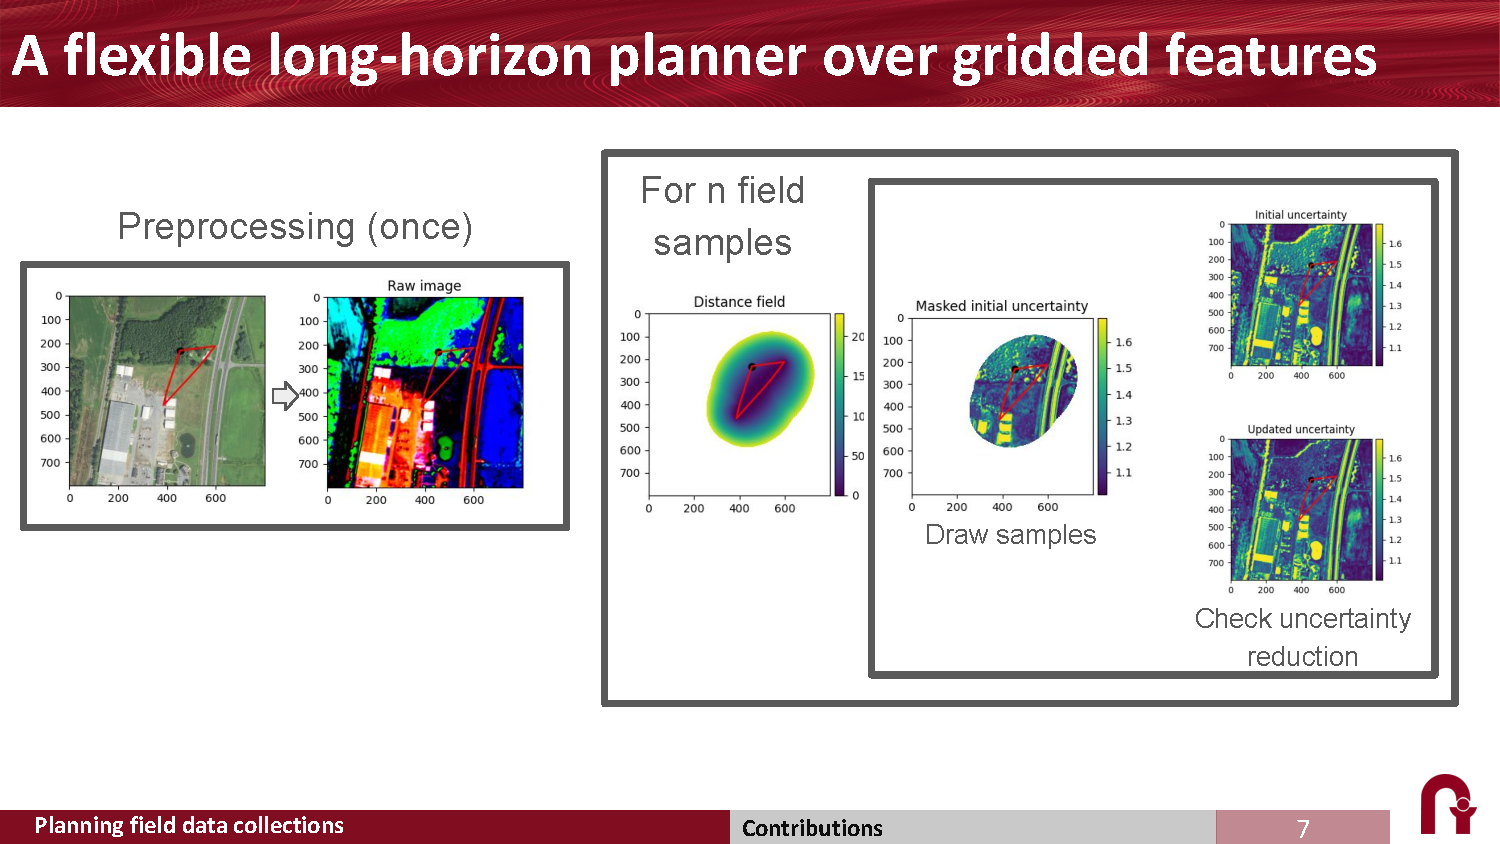
\includegraphics[width=\textwidth]{figs/methods/IPP/RAPTORS_concept.pdf}
    \caption{RAPTORS overview}
    \label{fig:methods:IPP_raptors_overview}
\end{figure}

\begin{itemize}
    \item We employ a sampling-based strategy to build a long horizon offline path. This takes in an initial location, a number of samples, and a traversal budget. The algorithm begins by computing the gaussian process uncertainty after only observing the first location. Then, a feasible region is computed using a fraction of the remaining budget. A fixed number of samples are drawn from this feasible region, using a weighted sampling based on their uncertainty. The sample which reduces the total map unceratinty the most is added to the plan. Then the points are ordered using a TSP solver. The feasible region is recomputed using the added points and the fraction of the remaining budget.
\end{itemize}